\documentclass{article}
\usepackage[utf8]{inputenc}
\usepackage{setspace}
\usepackage{amsmath}
\usepackage{enumerate}
\usepackage{enumitem}
\usepackage{moreenum}
\usepackage{multirow}
\usepackage[greek,english]{babel}
\usepackage{alphabeta}
\usepackage{tabularx}
\usepackage{graphicx}
\usepackage{hyperref}

\begin{document}
\begin{center}

\large{\textbf{Δεύτερη υποχρεωτική εργασία στην αριθμητική ανάλυση}}\\
\large{\textbf{Ονοματεπώνυμο: Νικόλαος Βογιατζής} \textbf{ΑΕΜ: 3952}}\\

\large{\textbf{Ημερομηνία Παράδοσης: 21/01/2022}}\\
\end{center}

\large{\textbf{Άσκηση 5:}}\\
Ο κώδικας για την άσκηση 5 βρίσκεται στον φάκελο "Code" και είναι το αρχείο ex5.py.\\
Στην άσκηση αυτή καλούμαστε να υπολογίσουμε το ημίτονο οποιασδήποτε γωνίας στο $[-\pi, \pi]$ με 10 αρχικά - μη-ομοιόμορφα κατανεμημένα σημεία με τις μεθόδους: Πολυωνυμικής προσέγγισης (χρησιμοποιήθηκε το πολυώνυμο Lagrange), με τη μέθοδο Splines και
τη μέθοδο των ελαχίστων τετραγώνων. Στον κοινό κώδικα (main) για τις 3 μεθόδους βρίσκονται: Η αρχικοποίηση των 10 αρχικών σημείων και η αποθήκευσή τους στη λίστα x\_values, ο υπολογισμός των
$f(x_i) $ για κάθε x\_value[i] και η αποθήκευση των αποτελεσμάτων στη λίστα y\_values. Έπειτα καλούνται οι τρεις συναρτήσεις που καλούν τις αντίστοιχες μεθόδους και τυπώνονται τα αποτελέσματα. \\
Ως αρχικά σημεία επιλέχθηκαν τα: x0 = $-\pi$ , x1 = $-\dfrac{\pi}{2}$ , x2 = $-\dfrac{\pi}{4}$, x3 = $-\dfrac{\pi}{6}$, x4 =$-\dfrac{\pi}{8}$ , x5 = 0 , x6 =$\dfrac{\pi}{7}$ , x7 =$\dfrac{\pi}{4}$ , x8 =$\dfrac{\pi}{2}$ , x9 =$\pi$.
\par\textbf{Πολυωνυμική προσέγγιση:}\\

\par
Στην συνάρτηση που επιλύει την άσκηση με το πολυώνυμο Lagrange, αρχικοποιείται το αποτέλεσμα που θα επιστραφεί, σε 0. Έπειτα σε μία επανάληψη n φορών , όπου $n = len(x\_data)$ αρχικοποιείται η μεταβλητή Lx σε y\_values[i] και σε μία δεύτερη επανάληψη n φορών υπολογίζεται ο τύπος του πολυωνύμου
\begin{center}
$L_i(x) = \dfrac{(x-x_0)...(x - x_{i-1})(x-x_{i+1})...(x-x_n)} {(x_i - x_0)...(x_i - x_{i-1})(x_i - x_{i+1})...(x_i - x_n)}$
\end{center}και πολλαπλασιάζεται με το Lx (στην πρώτη επανάληψη, με την τιμή του Lx που αρχικοποιήθηκε έξω από την δεύτερη επανάληψη, σε κάθε άλλη επανάληψη με την προηγούμενη τιμή που είχε το Lx). Όσα αφορούν την δεύτερη επανάληψη συμβαίνουν μόνο όταν οι μετρητές των δύο επαναλήψεων δεν είναι ίδιοι. Αν είναι ίδιοι τότε η δεύτερη επανάληψη προχωρά στην επόμενή της επανάληψη. Όταν τελειώσει η εμφωλευμένη επανάληψη, η τιμή της Lx προστίθεται στο αποτέλεσμα. Τέλος επιστρέφεται το αποτέλεσμα (result).
\par\textbf{Splines:}\\
Για την προσέγγιση του ημιτόνου με τη μέθοδο Splines, χρησιμοποιήθηκαν οι πίνακες τετμημένων, τεταγμένων που χρησιμοποιήθηκαν και στην πολυωνυμική προσέγγιση. Η μέθοδος υλοποιήθηκε βάσει της φυσικής κυβικής spline. Η συνάρτηση που υλοποιεί τη μέθοδο είναι η Splines(x, x\_data, y\_data). Μέσα σε αυτή, ορίζουμε τη λίστα delta[length\_of\_subspaces] ως το μήκος των υποδιαστημάτων μεταξύ x\_i και x\_{i+1}. Αποθηκεύουμε κάθε μήκος σε ένα κελί του πίνακα (λίστα) delta[length\_of\_subspaces], με length\_of\_subspaces το πλήθος των υποδιαστημάτων (για 10 σημεία 9 υποδιαστήματα). Έπειτα στον πίνακα second\_derivatives[length\_of\_subspaces -1], αποθηκεύουμε την τιμή της δεύτερης παραγώγου που προκύπτει από τον τύπο 
\begin{equation}
    3\left(\dfrac{ y\_data_{i+2} - y\_data_{i+1}}{delta[i+1]} -  \dfrac{ y\_data_{i+1} - y\_data_i}{delta[i]}\right)
\end{equation} \\
Ορίζουμε τρεις λίστες lower\_diagonal[n], upper\_diagonal[n], main\_diagonal[n], με n το πλήθος των τετμημένων, που συμβολίζουν την κάτων, πάνω και κύρια διαγώνιο του τριδιαγώνιου συστήματος που καλούμαστε να λύσουμε. Όλες οι λίστες αρχικοποιούνται με 0 σε κάθε κελί κι έπειτα ορίζουμε την τιμή στο πρώτο κελί να είναι 1 και 0 για την κάτω διαγώνιο και την κύρια, αντίστοιχα. Σε μία επαναληπτική μέθοδο από 1 ως
length\_of\_subspaces , υπολογίζουμε τις τιμές των τριών διαγωνίων σύμφωνα με τους τύπους.
\begin{equation*}
    lower\_diagonal = 2(x\_data[i+1] - x\_data[i -1]) - delta[i-1]upper\_diagonal[i-1]
\end{equation*}

\begin{equation*}
    upper\_diagonal = \dfrac{delta[i]}{lower\_diagonal[i]}
\end{equation*}
    
\begin{equation*}
    main\_diagonal = \dfrac{(second\_derivatives[i-1] - delta[i-1] * main\_diagonal[i-1]}{lower\_diagonal)}
\end{equation*}
Η παραπάνω επαναληπτική μέθοδος ορίζει το τριδιαγώνιο σύστημα.
Όταν ολοκληρωθεί το παραπάνω βήμα, ορίζουμε b[n], c[n], d[n] λίστες (σε 0), οι οποίες συμβολίζουν τις λύσεις του τριδιαγώνιου συστήματος. Δηλαδή χρησιμοποιούμε μία επανάληψη από την τελευταία προς την πρώτη γραμμή, και βρίσκουμε τις τιμές των τριών πινάκων σύμφωνα με τους τύπους:
\begin{equation*}
    c[i] = main\_diagonal[i] - upper\_diagonal[i]c[i+1]
\end{equation*}

\begin{equation*}
    b[i] = \dfrac{(y\_data[i+1] - y\_data[i])}{delta[i]}  - delta[i]\dfrac{(c[i + 1] +2c[i])}{3}
\end{equation*}

\begin{equation*}
    d[i] = \dfrac{(c[i+1]) - c[i]}{3delta[i]}
\end{equation*}
Τέλος αφού είναι γνωστά πλέον τα b,c,d σε μία επανάληψη για κάθε υποδιάστημα ελέγχουμε αν η τιμή του χ που δόθηκε από τον χρήστη είναι μεταξύ κάποιου από τα υπάρχοντα υπο-υποδιαστήματα κι αν ναι επιστρέφεται ως αποτέλεσμα η τιμή του πολυωνύμου της φυσικής κυβικής splines: $y_i + b_i(x-x_i) + c_i(x - x_i)^2 + d_i(x-x_i)^3$
\par\textbf{Ελάχιστα Τετράγωνα:}\\
Για την προσέγγιση του ημιτόνου με τη μέθοδο των ελαχίστων τετραγώνων, χρησιμοποιήθηκε η τετραγωνική καμπύλη. Έτσι προσπαθούμε με διαδοχικά βήματα να χτίσουμε το πολυώνυμο $y = a + bx + cx^2$. Γίνεται η χρήση των σημείων και των λιστών που χρησιμοποιήθηκαν και στις προηγούμενες μεθόδους (x\_values, y\_values). Η συνάρτηση που υλοποιεί την μέθοδο είναι η Least\_Squares(x, x\_array, y\_array). Αρχικά, δηλώνονται-αρχικοποιούνται όλοι οι πίνακες που θα χρειαστούμε, σε μορφή nested list , δηλαδή οι:
A[10][3], ο πίνακας που περιέχει άσσους στην πρώτη στήλη, τις τιμές των τετμημένων στη δεύτερη και τις τιμές των τετμημένων στο τετράγωνο στη τρίτη στήλη, AT[3][10], ο ανάστροφος του πίνακα Α, AT\_A[3][3], που είναι ο πίνακας που θα προκύψει από τον πολλαπλασιασμό του ανάστροφου AT με τον αρχικό πίνακα Α, b[10], ο πίνακας με στοιχεία τα y\_arrray[i] και ο ΑΤ\_b[10], ο πίνακας που προκύπτει από τον πολλαπλασιασμό του ανάστροφου του Α (ΑΤ) με τον πίνακα-διάνυσμα b. Οι παραπάνω πίνακες αρχικοποιούνται με 0 σε κάθε κελί. Έπειτα υπολογίζεται ο πίνακας Α[10][3] και ο b[10] και το επόμενο βήμα είναι ο υπολογισμός των AT\_A και AT\_b, οι οποίοι υπολογίζονται με την βοήθεια εμφωλευμένων "for" loops. Όταν πλέον έχουμε τους πίνακες γεμάτους, με την built-in συνάρτηση (linalg.solve)της βιβλιοθήκης numpy, λύνουμε το σύστημα AT\_Ax = AT\_b, όπου το διάνυσμα x είναι το διάνυσμα των αγνώστων και μάλιστα το αποτέλεσμα που επιστρέφει η συνάρτηση numpy.linalng.solve(AT\_A, AT\_b). Τώρα που το διάνυσμα είναι γνωστό, αποθηκεύουμε σε τρεις μεταβλητές a,b,c το αποτέλεσμα του αντίστοιχου αγνώστου και επιστρέφουμε την τιμή $a + bx + cx^2$ , όπου x ο αριθμός που δίνεται σαν είσοδος από τον χρήστη.

\par\textbf{Υποθέσεις-Επεξηγήσεις σχετικά με τη γραφική παράσταση των μεθόδων!}\\
Για την προσέγγιση του ημιτόνου και συνεπώς την υλοποίηση των παραπάνω μεθόδων, έγινε η υπόθεση πως
κάθε τιμή (τετμημένων-τεταγμένων) έχει ακρίβεια ακριβώς έξι δεκαδικών ψηφίων. Για να επιτευχθεί αυτό έγινε στρογγύλευση με αποκοπή χρησιμοποιώντας τη συνάρτηση round(x,6) της python. Για την προβολή των σφαλμάτων των τριών μεθόδων για 200 σημεία στο διάστημα $[-\pi, \pi]$, εργάστηκα ως εξής. Δημιούργησα 2 λίστες μεγέθους 200, μία για τις τετμημένες (x\_points[200]) και μία για τις τεταγμένες (y\_points[200]). Η πρώτη τετμημένη είναι το $-\pi$ και η τελευταία το $\pi$. Ορίζεται ένα βήμα (step = $\dfrac{\pi}{100}$) μέσω του οποίου η επόμενη τετμημένη μίας άλλης τετμημένης, έχει την τιμή της προηγούμενης συν το βήμα. Έπειτα σε 3 διαφορετικές επαναληπτικές μεθόδους, υπολογίζεται η τιμή των τεταγμένων βάσει των τριών μεθόδων αντίστοιχα, με γνωστά σημεία τα 10 σημεία που χρησιμοποιήθηκαν στις παραπάνω υλοποιήσεις και τα αποτελέσματα αποθηκεύονται σε 3 λίστες που αντιστοιχούν σε κάθε μέθοδο. Τέλος σε μία επανάληψη για κάθε ένα από τα 200 σημεία, υπολογίζεται η διαφορά της πραγματικής τιμής του ημιτόνου για το σημείο αυτό μείον την τιμή που βρήκε η κάθε μέθοδος και για τα σημεία που η διαφορά είναι 0 αυξάνεται ένας μετρητής για κάθε μέθοδο. Τέλος εμφανίζονται τα αποτελέσματα τα οποία είναι:\\
\begin{itemize}
    \item Lagrange  57 σημεία ακριβείας
    \item Splines 7 σημεία ακριβείας
    \item Ελάχιστα τετράγωνα  0 σημεία ακριβείας (στην πραγματικότητα είναι 3 τα σημεία και φαίνονται στην παρακάτων γραφική παράσταση, απλώς λόγω του τρόπου με τον οποίο επιλέχθηκαν τα 200 σημεία, δεν βρίσκονται μέσα σ'αυτά.)
\end{itemize}

Η γραφική παράσταση του σφάλματος της κάθε μεθόδου για τα 200 σημεία από την πραγματική γραφική παράσταση του ημιτόνου είναι η εξής: \\

\begin{center}
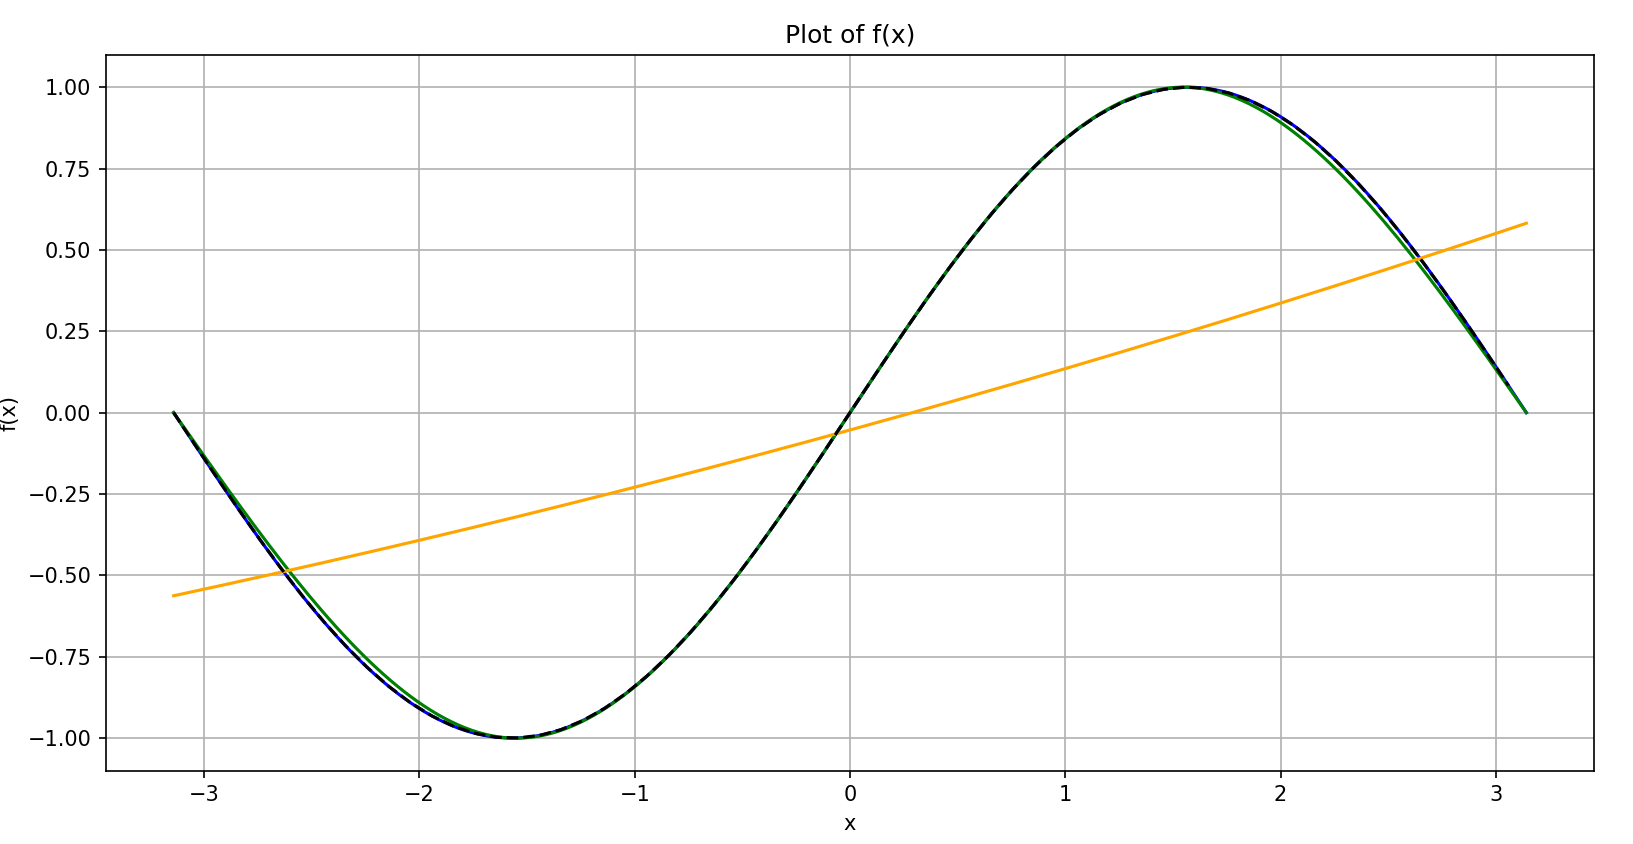
\includegraphics[width=.9\linewidth]{Plot.png}
\end{center}
Στο παραπάνω σχήμα, με κίτρινο χρώμα είναι η προσέγγιση με τα ελάχιστα τετράγωνα, με πράσινο η προσέγγιση με Splines, με μπλε η Lagrange και με διακεκομμένες και μαύρο χρώμα είναι η αυθεντική γραφική παράσταση του ημιτόνου x. Δεν είναι τόσο ευδιάκριτο το σφάλμα που προκύπτει για κάθε μέθοδο αλλά με ζουμ στη γραφική παράσταση παρατηρούμε ότι η Lagrange βρίσκεται αρκετά κοντά στην πραγματική, η Splines είναι μία πολύ καλη προσέγγιση αλλα όχι όπως η πολυωνυμική και για την μέθοδο των ελαχίστων τετραγώνων είναι φανερό ότι δεν προσεγγίζει με καλή ακρίβεια το ημίτονο. Αυτά φαίνονται εδώ.

\begin{center}
    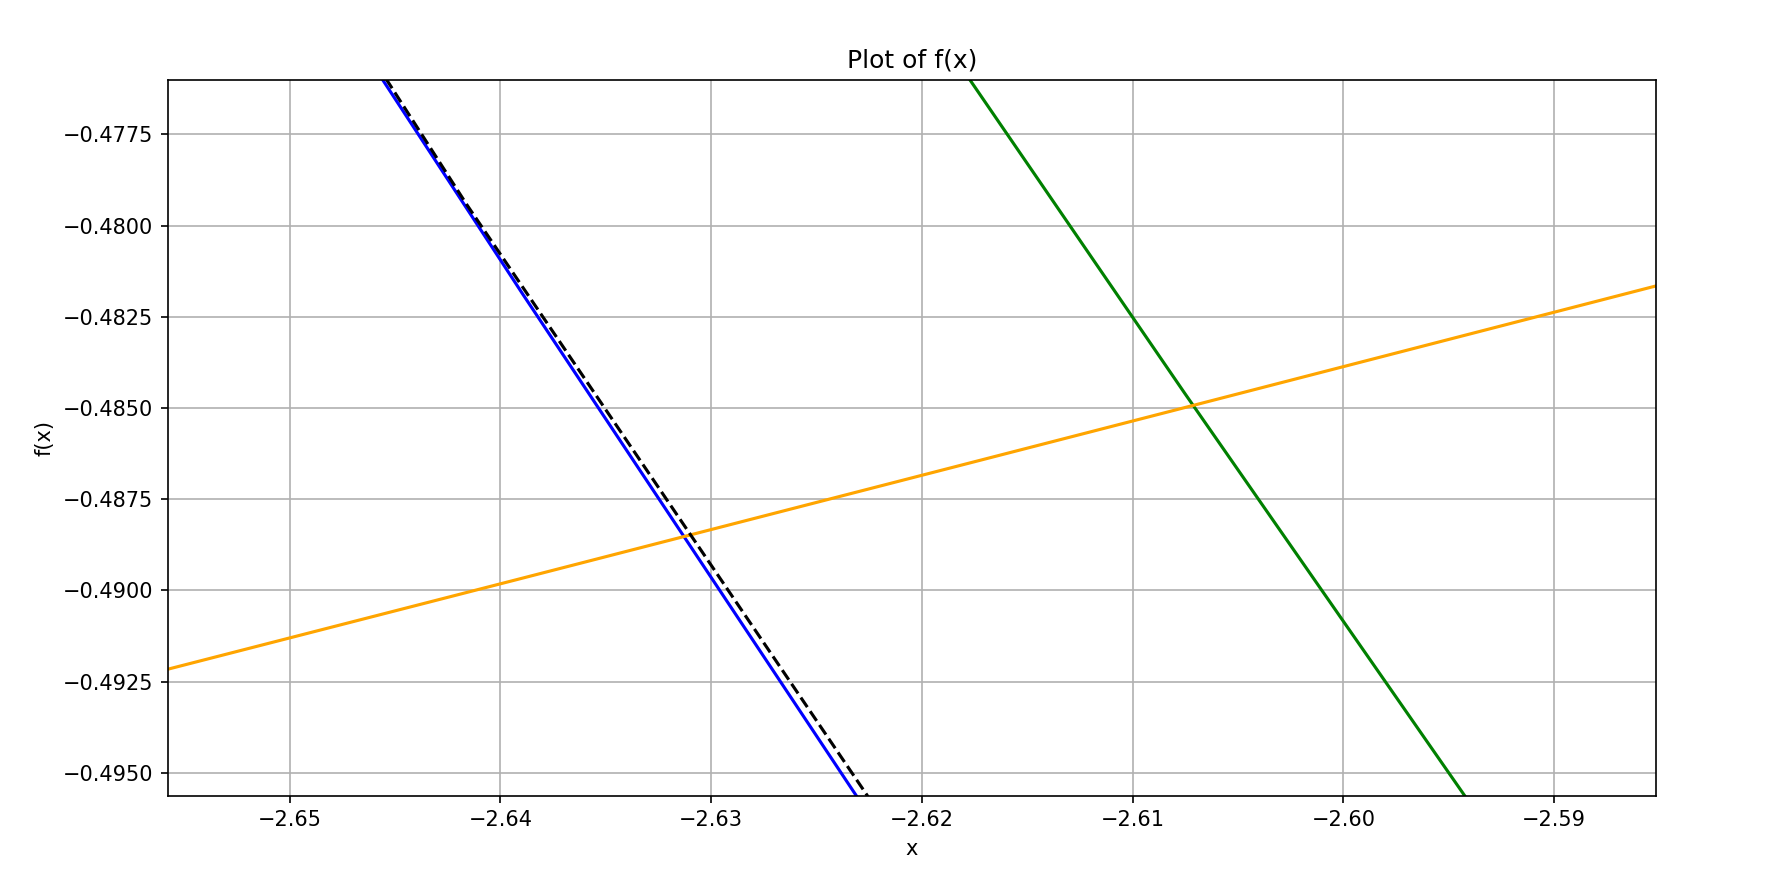
\includegraphics[width=.9\linewidth]{zoomed.png}
\end{center}
\par\textbf{Άσκηση 6:}
Ο κώδικας για την άσκηση 6 βρίσκεται στον φάκελο "Code" και είναι το αρχείο ex6.py.\\
Στην άσκηση αυτή καλούμαστε να υπολογίσουμε το ολοκλήρωμα της συνάρτησης sin(x) στο διάστημα 
$[$0$, \dfrac{\pi}{2}]$ χρησιμοποιώντας: Τη μέθοδο του \textbf{τραπεζίου} και τη μέθοδο \textbf{Simpson} 
και 11 αρχικά σημεία της επιλογής μας. Έπειτα να υπολογίσουμε και να αναφέρουμε το θεωρητικό και το 
πραγματικό σφάλμα.\\

\par\textbf{Μέθοδος Τραπεζίου} \\
Για την μέθοδο του τραπεζίου, όπως και για την μέθοδο Simpson , αρχικοποιούνται ως global μεταβλητές,
τα άκρα του διαστήματος $a = 0$ , $b = \dfrac{\pi}{2} $ και $N=10$ το μέγεθος των υποδιαστημάτων που
θα χρειαστούμε, αφού μας δίνεται ότι ξεκινάμε με 11 σημεία. Αρχικά υπολογίζονται τα 11 σημεία 
σύμφωνα με τον τύπο: $ x_i = κ\dfrac{b-a}{N} $, όπου κ=0,1,...,N και αποθηκεύονται σε μία λίστα
x\_values. Έπειτα υπολογίζουμε τις τιμές της $f(x)$ για κάθε x που υπολογίσαμε και το
αποθηκεύουμε σε μία λίστα y\_values. Τέλος, καλούμε τη συνάρτηση Trapezodial\_Method(y\_values) η οποία μας επιστρέφει: Την προσεγγιστική τιμή
του ολοκληρώματος, το θεωρητικό σφάλμα, το πραγματικό σφάλμα.\\
Στη συνάρτηση αυτή, αρχικοποιόυμε τις μεταβλητές integral και Sigma σε μηδέν.
Σε μία επανάληψη για N, υπολογίζουμε το Sigma σύμφωνα με
τον τύπο $\sum_{k=1}^{N-1} f(x_k)$. Η προσεγγιστική τιμή του ολοκληρώματος προκύπτει από τον 
τύπο $ \dfrac{b-a}{2N}\left(f(x_0) + f(x_N) + 2Sigma \right)$. Εφαρμόζοντας τα παραπάνω λαμβάνουμε ως ολοκλήρωμα της $f(x) = \sin{x}$ στο
[$0,\dfrac{\pi}{2}$] το 0.9979429863543572. \\Το θεωρητικό σφάλμα προκύπτει από τον τύπο
$ \dfrac{\left(b-a\right)^3}{12N^2} M$, όπου Μ= $ \max_{x\epsilon [a,b]}|f''(x)|: x\epsilon [a,b]$ με τιμή 1 αφού $ \int_{0}^{\dfrac{\pi}{2}} -sin{x} \,dx =  \cos{x} \big|_0^\dfrac{\pi}{2}$ = $0 - (1) = -1$ και κατ' απόλυτο τιμή ίσο με 1. Έτσι το θεωρητικό σφάλμα ισούται με 0.0020570136456428134. Το πραγματικό σφάλμα ισούται με 0.0032298204875312307. Το πραγματικό σφάλμα
υπολογίζεται ως εξής:  $|$ πραγματική τιμή ολοκληρώματος - προσεγγιστική τιμή $|$ .Η πραγματική τιμή του ολοκληρώματος είναι γνωστό πως είναι ίση με 1 αφού $ \int_{0}^{\dfrac{\pi}{2}} sin{x} \,dx =  -\cos{x} \big|_0^\dfrac{\pi}{2}$ = $0 - (-1) = 1$ .Άρα το πραγματικό σφάλμα είναι 
$\lvert 1 - 0.9979429863543572\rvert = 0.0032298204875312307 $ 
\par\large\textbf{Μέθοδος Simpson:}\\
Για τη μέθοδο Simpson οι αρχικοποιήσεις όσον αφορά τα x\_values και y\_values γίνονται με τον ίδιο τρόπο. Κι εδώ για τον υπολογισμό τόσο του ολοκληρώματος όσο και των σφαλμάτων, χρησιμοποιείται μία συνάρτηση, η Simpson(x\_values). Αρχικά υπολογίζονται οι δύο σειρές με τύπους
sigma1 = $\sum_{i=1}^{\dfrac{N}{2}-1}$ $f(x_{2i})$  και \\
sigma2 = $\sum_{i=1}^{\dfrac{N}{2}} f(x_{2i-1})$. Έπειτα η προσεγγιστική τιμή του ολοκληρώματος υπολογίζεται από τον τύπο $ \dfrac{b-a}{3N}\left(f(x_0) + f(x_N) + 2Sigma1 + 4Sigma2 \right)$ και ως αποτέλεσμα παίρνουμε το 1.0000033922209004.
Για το θεωρητικό σφάλμα, χρησιμοποιήθηκε ο τύπος $\|e\| \leq \dfrac{\left(b-a\right)^2}{180N^4}M$ με \\
$M= max_{x\epsilon [a,b]}|f^{(4)}(x)|: x\epsilon [a,b]$ , το οποίο ισούται με 1 αφού
$\int_0^{\dfrac{\pi}{2}} \sin{x} \,dx = 1 $ (όπως παραπάνω).  Με την υλοποίηση των παραπάνω, λαμβάνουμε στην έξοδο την τιμή του θεωρητικού σφάλματος ίση με 5.312841749744469e-06. Το πραγματικό σφάλμα είναι πάλι η πραγματική τιμή του ολοκληρώματος - την προσέγγισή μας κατ' απόλυτο τιμή. Ισούται με  3.3922209004000337e-06.

\end{document}
